%! Tex program = xelatex
\documentclass[UTF8]{article}
\usepackage{indentfirst}
\usepackage{graphicx} 
\usepackage{amsmath}  
\usepackage{float}   
\usepackage{listings}

\title{Discrete Mathematics}
\author{Zhengren Wang 2019081308021}
\date{06/02/2020 Tue}
\begin{document}
\maketitle 

\part{10.3}
\begin{description}
    \item[15]Represent the given graph using an adjacency matrix. \\
        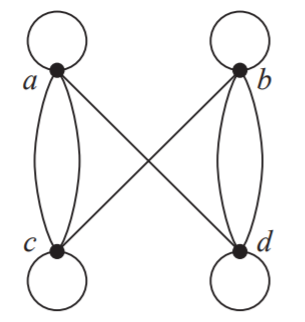
\includegraphics[scale=0.3]{../imgs/10_3_15.png}   \\
        $\begin{bmatrix}
            1 & 0 & 2 & 1   \\
            0 & 1 & 1 & 2   \\
            2 & 1 & 1 & 0   \\
            1 & 2 & 0 & 1   \\
        \end{bmatrix}$



    \item[39]Determine whether the given pair of graphs is isomorphic. Exhibit an isomorphism or provide a rigorous argument that none exists  \\
        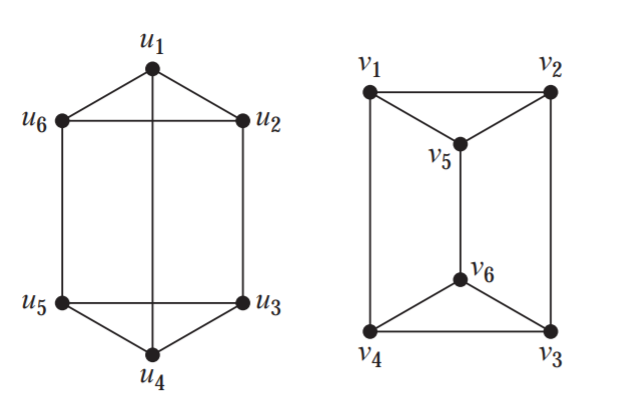
\includegraphics[scale=0.3]{../imgs/10_3_39.png}      \\
        They are isomorphic. \\
        We can prove it by transform $u_1 \to v_5, u_4 \to v_6, u_6 \to v_1, u_2 \to v_2, u_5 \to v_4, u_3 \to v_3$.  \\

    \item[45]Show that isomorphism of simple graphs is an equivalence relation. \\\\
            Reflexivity  : $G$ is isomorphic to itself by the identity function, so isomorphism is reflexive.   \\\\
            Symmetry     : Suppose that $G$ is isomorphic to $H$. Then there exists a one-to-one correspondence $f$ from $G$ to $H$. It follows that $f^{−1}$ is also a one-to-one correspondence from $H$ to $G$. Therefore, isomorphism is symmetric.    \\\\
            Transitivity : If $G$ is isomorphic to $H$ and $H$ is isomorphic to $Q$, then there are one-to-one correspondences $f$ and $g$ from $G$ to $H$ and from $H$ to $Q$. It follows that $g\circ f$ is also one-to-one from $G$ to $Q$. Therefore, isomorphism is transitive    \\\\
            Conclusion   : Isomorphism is a kind of equivalence relation. \\\\
\end{description}

\end{document}
